\section{Requerimientos previos \label{sec:reqPrevios}}
Los requerimientos previos se consideran para la compilación del sistema en
\texttt{Ubuntu 22.04.3 LTS}, entonces se coloca en esta sección las instrucciones 
para dicha distribución.

\subsection{Instalación de herramientas}
	Debido a que \texttt{GN} utiliza \texttt{Ninja} y, en general, para la 
	compilación del \textit{kernel} se utilizan las utilidades de GNU y otras
	librerías de desarrollo, es conveniente instalar todas estas herramientas antes de continuar a los requerimientos posteriores.
	
	
	
	En el repositorio del autor se menciona, en el archivo \texttt{docs/build.md}, sección \textit{Tools for Linux (Ubuntu)}, que las
	herramientas se instalan por medio de:
	\begin{center}
		\ttfamily
		apt install build-essential curl libmpfr-dev libmpc-dev libgmp-dev e2fsprogs qemu-system-i386 qemu-utils nasm fuseext2 ninja,
	\end{center}

	
	
	sin embargo, funciona mejor utilizar lo siguiente:
	\begin{center}
		\ttfamily
		sudo apt install build-essential curl libmpfr-dev libmpc-dev libgmp-dev e2fsprogs nasm fuseext2 ninja-build.
	\end{center}

	
	
	Por otro lado, se require también la instalación de \texttt{Python}, la distribución donde se compiló \texttt{OpuntiaOS}, así como otras recientes, ya lo
	traen instalado por defecto, sin embargo, puede instalarse como:
	\begin{center}
		\ttfamily
		sudo apt install python3.
	\end{center}


\subsection{Instalación de QEMU \label{ssec:installQuemu}}
	De acuerdo con el repositorio del autor (\texttt{docs/getting\_qemu.md}), debe 
	instalarse el emulador \texttt{QEMU} por medio de la siguiente línea:
	\begin{center}
		\ttfamily
		apt install qemu-utils qemu-system-i386 qemu-system-x86\_64 qemu-system-arm,
	\end{center}

	
	
	sin embargo, en la versión donde se llevó a acabo la compilación se debe 
	instalar como sigue:
	\begin{center}
		\ttfamily
		sudo apt install qemu-utils qemu-system-x86 qemu-system-arm.
	\end{center}

	
	De esta manera se tendrán disponibles las siguientes instrucciones 
	del sistema:
	\begin{itemize} \setlength\itemsep{0pt}
		\item \textbf{\texttt{qemu-system-x86\_64}},
		\item \textbf{\texttt{qemu-system-i386}},
		\item \texttt{qemu-system-aarch64},
		\item \textbf{\texttt{qemu-system-arm}}.
	\end{itemize}



\subsection{Instalación de GN \label{ssec:installGn}}
	\texttt{OpuntiaOS} utiliza GN como sistema de construcción, para instalarlo debe obtenerse su código fuente, el enlace se menciona tanto en el repositorio de
	\texttt{OpuntiaOS} (\texttt{docs/getting\_gn.md}) como en \cite{gn}.
	
	
	
	En el repositorio de \texttt{OpuntiaOS} se hace uso del comando \texttt{python}, sin embargo, resulta mejor opción utilizar \texttt{python3}, o bien, hacer un enlace simbólico que apunte al binario de \texttt{python3}.
	
	
	
	Después de validar que \texttt{Python} está disponible, puede proceder la 
	instalación tal como menciona el archivo \texttt{docs/getting\_gn.md}.
	\begin{figure}[ht]
		\centering
		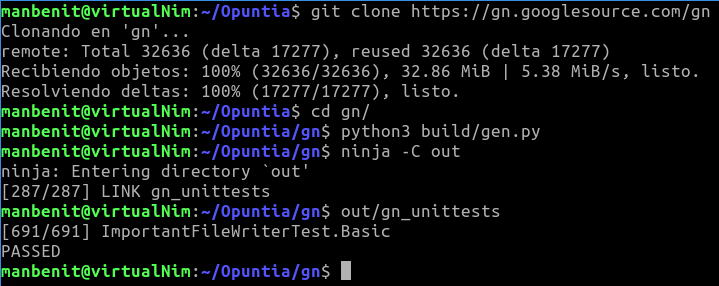
\includegraphics[scale=0.4]{installGn.png}
		\caption{
			Proceso de instalación de \texttt{GN}.
			\label{fig:installGn}
		}
	\end{figure}




\newpage
\subsection{Instalación de LLVM}
	Para instalar \texttt{LLVM} se requiere un archivo ejecutable que puede 
	conseguirse por medio de \texttt{wget}, esto se menciona en el repositorio de \texttt{OpuntiaOS} (\texttt{docs/build.md}).
	\begin{figure}[ht]
		\centering
		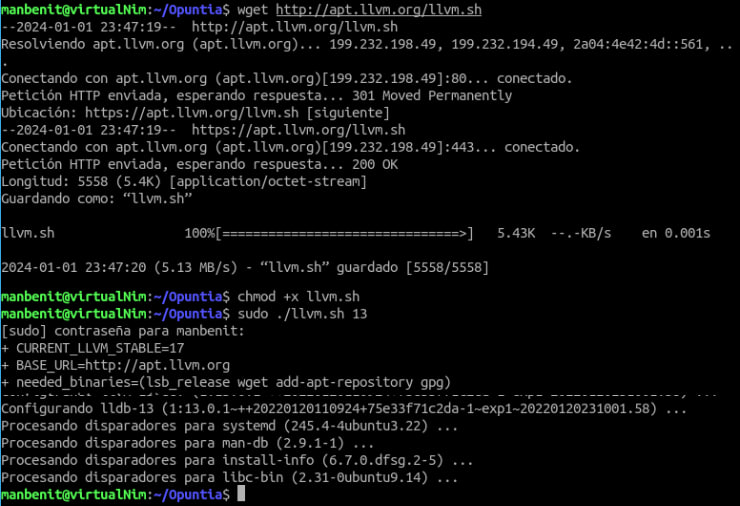
\includegraphics[scale=0.51]{installLlvm.jpg}
		\caption{
			Proceso de instalación de \texttt{LLVM}.
			\label{fig:installLlvm}
		}
	\end{figure}


\subsection{Instalación de dependencias de Python}
	En el archivo \texttt{docs/build.md} también se menciona la instalación de
	las dependencias:
	\begin{itemize} \setlength\itemsep{0pt}
		\item \texttt{construct}, versión 2.10.67,
		\item \texttt{gitpython}, versión 3.1.27,
		\item \texttt{pyelftools}, versión 0.28,
	\end{itemize}
	
	
	
	que se especifican en el archivo 
	\texttt{utils/python\_requirements.txt},
	y de la misma manera que en la \autoref{ssec:installGn}, se recomienda usar la versión reciente, en este caso, del gestor de paquetes (\texttt{pip3}), en lugar del \texttt{pip} mencionado en el repositorio.
	
	
\newpage
\subsection{Instalación del \textit{toolchain} para x86}
	Se deben asignar permisos de ejecución al \textit{script} de instalación por medio de 
	\begin{center}
		\ttfamily
		chmod 775 toolchains/scripts/i686-elf-tools.sh,
	\end{center}

	este archivo se referencia en \texttt{docs/build.md}, sección \textit{GNU Toolchain for Linux (Ubuntu)}, del repositorio de \texttt{OpuntiaOS}.
	
	
	
	El \textit{script} se encarga de:
	\begin{itemize} \setlength\itemsep{0pt}
		\item Guarda la ruta de construccion en HOME
		\item guarda la ruta de construcción en la variable de entorno del sistema.
		\item Instalar paquetes útiles para la compilación futura del sistema, varias de ellas es probable que ya vengan pre-instaladas por defecto.
		
	\end{itemize}

	En la función \texttt{installPackages} se intenta instalar \texttt{Python}, pero debe cambiarse el nombre del paquete a \texttt{python3}, porque en distribuciones recientes como en la que se compiló el sistema se utiliza la forma reciente (\texttt{python3}).
	\begin{figure}[ht]
		\centering
		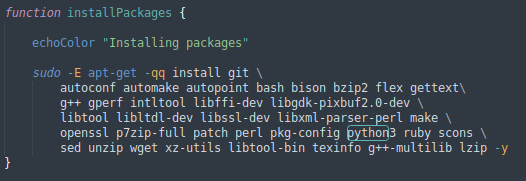
\includegraphics[scale=0.55]{modificarPython.png}
		\caption{
			Modificación de \texttt{python} a \texttt{python3} en la función \texttt{installPackages} de \texttt{i686-elf-tools.sh}.
			\label{fig:modificarPython}
		}
	\end{figure}

	\newpage
	
	Finalmente debe ejecutarse como indica el repositorio:
	\begin{center}
		\ttfamily
		./toolchains/scripts/i686-elf-tools.sh,
	\end{center}
	cuya ejecución se muestra en la \autoref{fig:toolchainx86}. El proceso tarda varios minutos.
	\begin{figure}[ht]
		\centering
		\subfloat[Proceso]{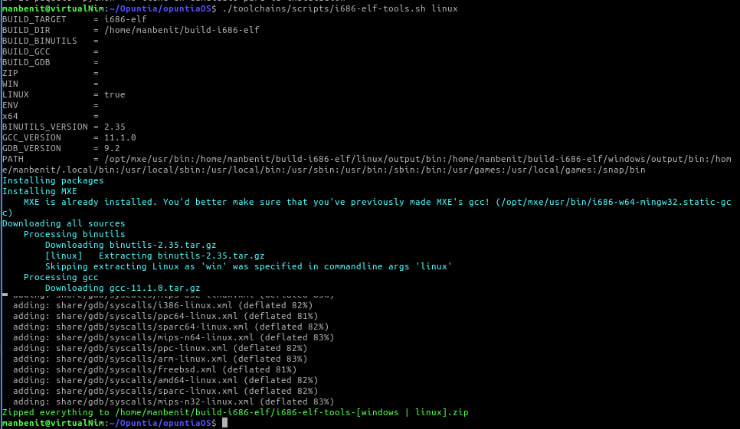
\includegraphics[scale=0.62]{toolchainx86.jpg}}
		\vspace{0.5cm}
		\subfloat[Resultado]{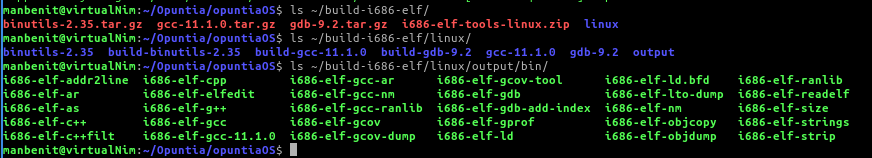
\includegraphics[scale=0.4]{toolchainx86_res.png}}
		\caption{
			Instalación del \textit{toolchain} para \texttt{x86}.
			\label{fig:toolchainx86}
		}
	\end{figure}

	
	
	Los binarios obtenidos de la instalación del \textit{toolchain} deben 
	agregarse a la variable de entorno del sistema (\texttt{PATH}) para
	su posterior uso en la construcción del sistema:
	\begin{center}
		\ttfamily
		export PATH=\$PATH:<directorio\_de\_contrucción>/linux/output/bin,
	\end{center}

	donde, \texttt{<directorio\_de\_contrucción>} es la ruta donde se 
	crea el \textit{toolchain}, por defecto se crea en \texttt{\$HOME}.
	
	
	
\newpage
\subsection{Instalación del \textit{toolchain} para ARM}
	Se deben asignar permisos de ejecución al \textit{script} de instalación por medio de 
	\begin{center}
		\ttfamily
		chmod 775 toolchains/scripts/arm-none-eabi-tools.sh,
	\end{center}

	este archivo se referencia en \texttt{docs/build.md}, sección \textit{GNU Toolchain for Linux (Ubuntu)}, del repositorio de \texttt{OpuntiaOS}.
	
	
	
	El \textit{script} se encarga de descargar y crear enlaces simbólicos a los binarios necesarios par ala compilación del sistema para \texttt{ARM}, sin embargo ocurren problemas debido a los nombres usados cuando se crean los enlaces simbólicos, además de hacer falta el \texttt{arm-none-eabi-objcopy}, necesario para la compilación, por lo que se recomienda modificar el \textit{script} como muestra la \autoref{fig:modifArmSsh}.
	\begin{figure}[ht]
		\centering
		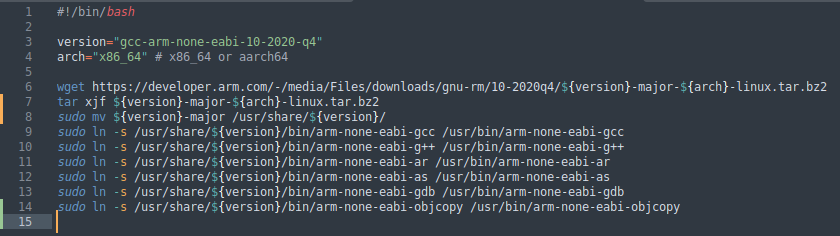
\includegraphics[scale=0.47]{modifArmSsh.png}
		\caption{
			Modificación del archivo \texttt{arm-none-eabi-tools.sh}.
			\label{fig:modifArmSsh}
		}
	\end{figure}
	
	\newpage
	
	Finalmente debe ejecutarse como indica el repositorio:
	\begin{center}
		\ttfamily
		./toolchains/scripts/arm-none-eabi-tools.sh,
	\end{center}
	cuya ejecución se muestra en la \autoref{fig:toolchainArm}.
	\begin{figure}[ht]
		\centering
		\subfloat[Proceso]{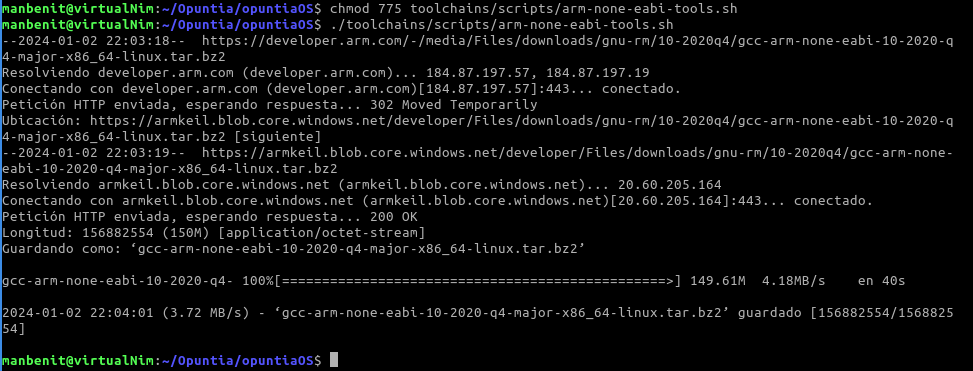
\includegraphics[scale=0.4]{toolchainArm.png}}
		\vspace{0.5cm}
		\subfloat[Resultado]{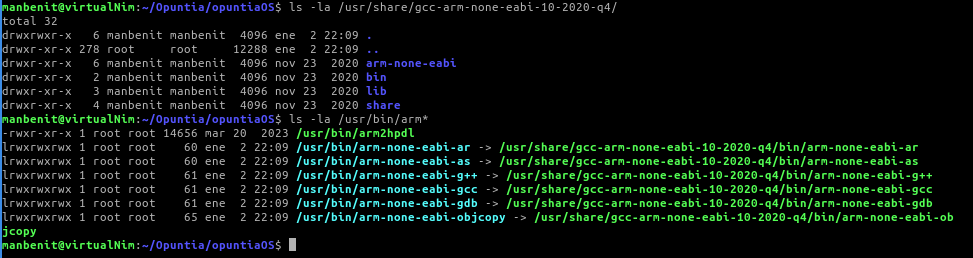
\includegraphics[scale=0.4]{toolchainArm_res.png}}
		\caption{
			Instalación del \textit{toolchain} para \texttt{ARM}.
			\label{fig:toolchainArm}
		}
	\end{figure}
	

